
\section{Introduction}

%proč OpenStack - protože komunita 500000 vývojářů, tisíce firem, nárůst kódu za poslední dobu stacalytics.com 

%vendor lockin, scalability from notebook to thousans of servers like CERN

OpenStack is the largest open-source cloud computing platform today. Many companies participate to its code, extend core functions and write new service backends to fit their business goals. The actual system consists of many components designed with plugin architecture that allows custom implementations for various service backends. These components can be combined and configured to match available software and hardware resources and real use-case needs.

Each implementation has its own component combination and use some form of configuration management tool to enforce the service states on designated servers and possibly other network components. These tools require data that covers configuration of all components. Detecting component inconsistencies by hand is painful and time consuming process.

We propose a formalization of OpenStack service architecture model, based on the approaches developed in classic knowledge representation domain, especially Service-Oriented Architecture by OpenGroup. Component definition is encoded in an ontology using the standard OWL-DL language, which enables sharing of knowledge about configurations across various systems. Reasoning can be used on the specification to automate validation of configuration changes.

When dealing with hundreds of components with thousands of properties and relations, keeping track of changes throughout its life cycle is very challenging. Current approaches are ad hoc, even OpenStack Fuel has severe limitations, there exists no standard for specifying common OpenStack architectural model. The question how to convert the proposed OWL-DL schema to metadata format that configuration management tools can process is discussed. We are working on external node classification service that uses graph database to serialize the OWL ontology with REST API that configuration management tools can use as metadata provider. This can streamline the process of adopting new services and service backends in predictable manner.

\begin{figure}[!h]
\centering
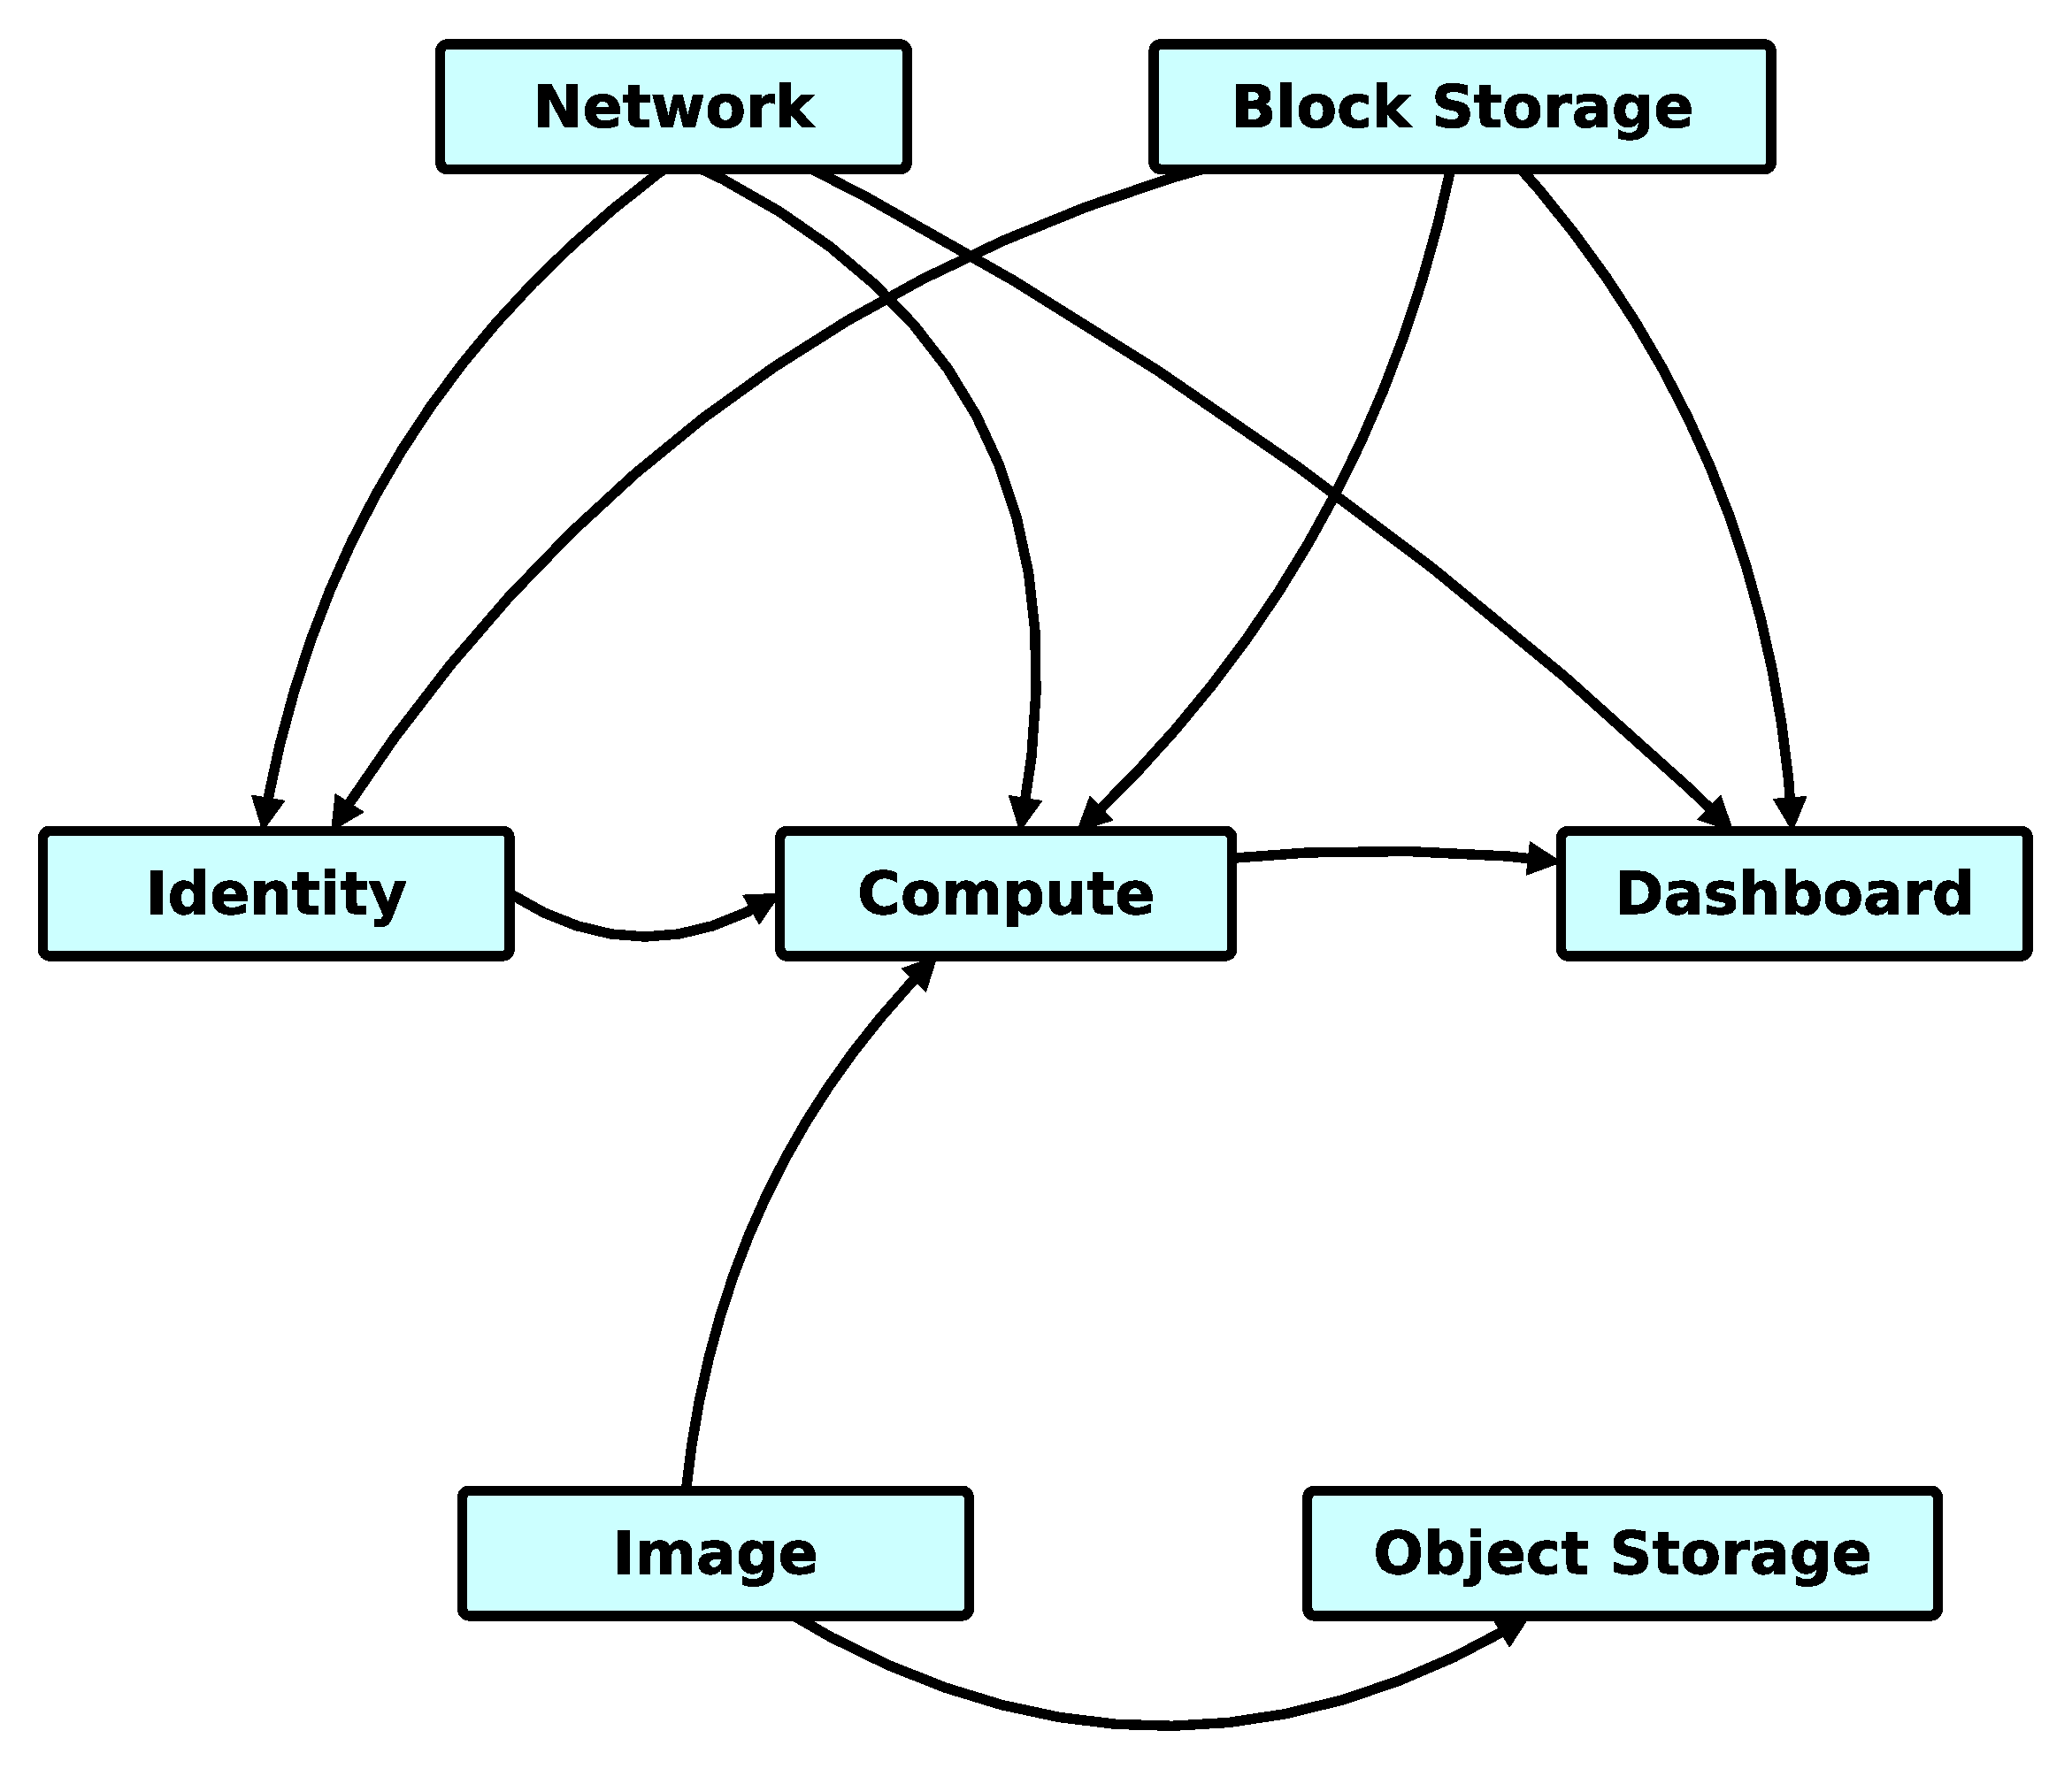
\includegraphics[scale=.2]{img/openstack_logical_model.eps}
\caption{Logical Model of Havana OpenStack}
\label{fig:cm}
\end{figure}


\begin{figure}[!h]
\centering
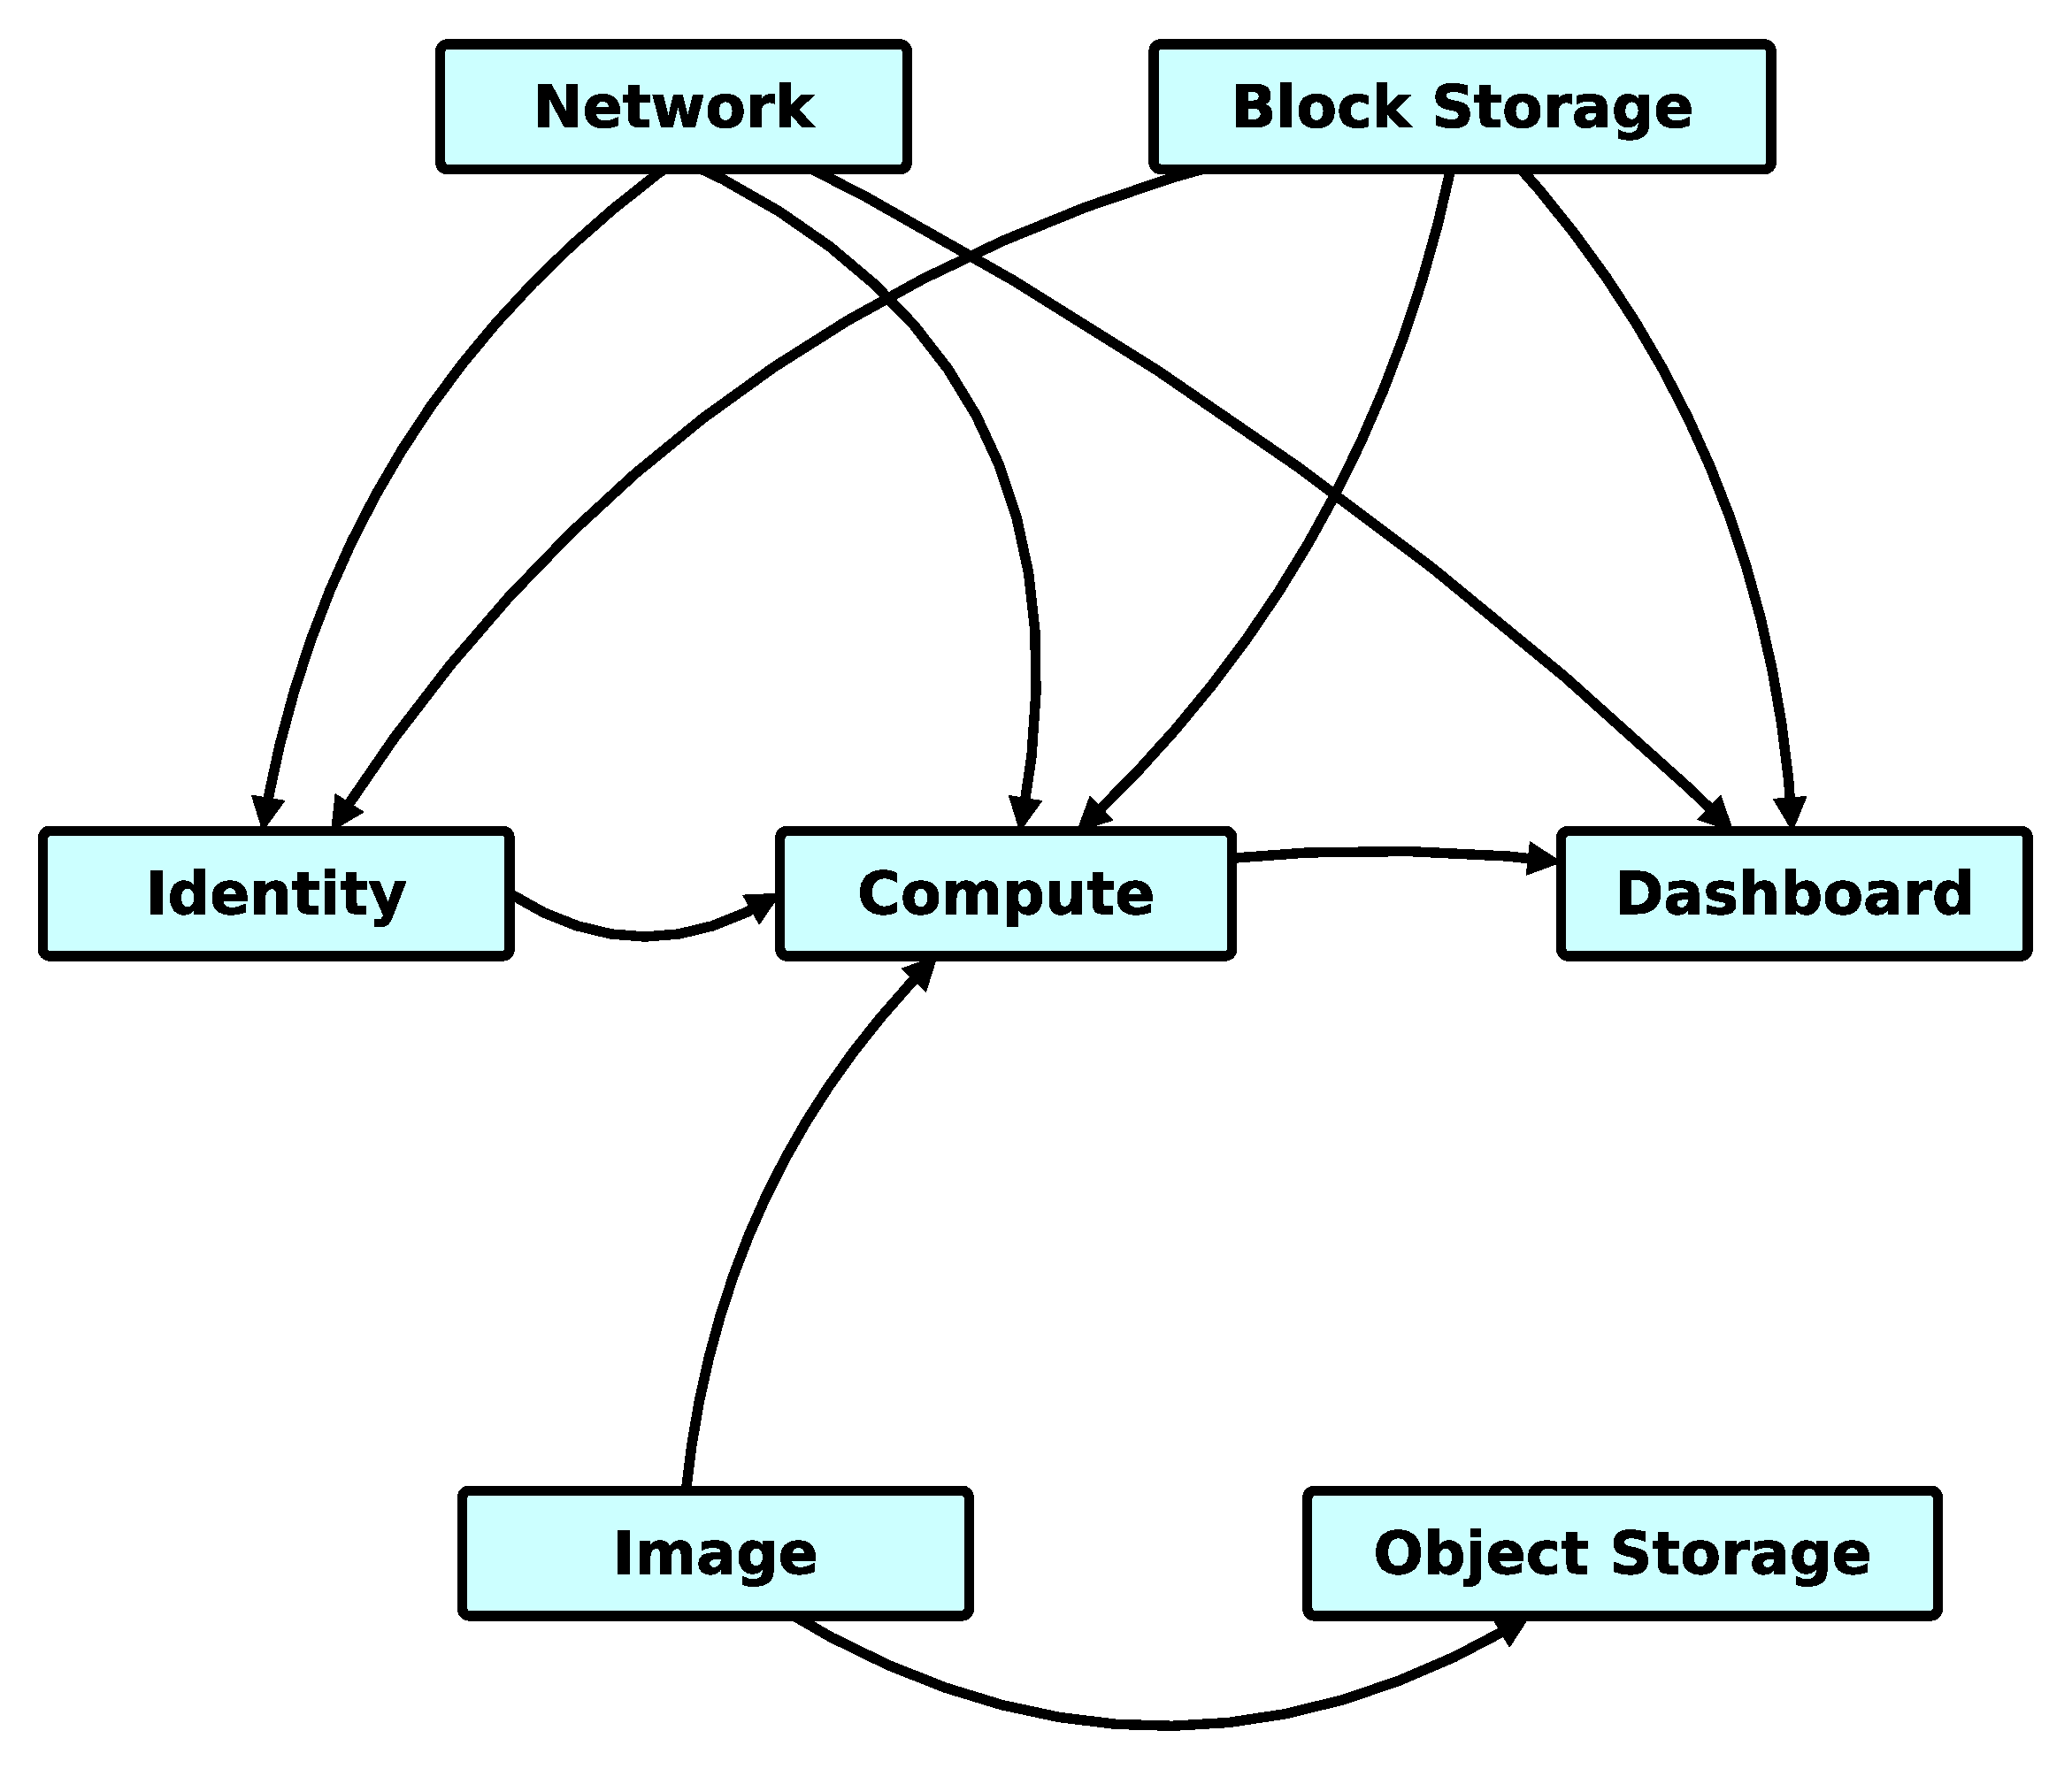
\includegraphics[scale=.2]{img/openstack_logical_model.eps}
\caption{Logical Model of Icehouse OpenStack}
\label{fig:cm}
\end{figure}


% představit OpenStack jako systém s rolemi, konfiguracemi, komponenty, drivery. jina instalace per use case. Nexexistuje univerzální instalace. Vysoka komplexita, services

% Jak vytvořit high level model (logické schéma) architektury? a přenést ji do low level design realizace? 
% Jak správně definovat architekturu na základě hw infrastruktury a target use case?

% Jak celý proces deploymentu automatizovat?

\subsection{IaaS Solutions}

\subsection{Use Cases}

\subsection{Infrastructure Modeling}
